\documentclass[../psets.tex]{subfiles}

\pagestyle{main}
\renewcommand{\leftmark}{Problem Set 7}
\setcounter{section}{7}

\begin{document}




\begin{enumerate}[label={\Roman*)}]
    \item \marginnote{3/5:}Do the following problems from Chapter 10: 13, 14, 27, 30, 33.
    \begin{enumerate}[label={\textbf{10.\arabic*}}]
        \setcounter{enumii}{12}
        \item Use the angular overlap method to calculate the energies of both ligand and metal orbitals for \emph{trans}-\ce{[Cr(NH3)4Cl2]+}, taking into account that ammonia is a stronger $\sigma$-donor ligand than chloride, but chloride is a stronger $\pi$ donor. Use the 1 and 6 positions for the chloride ions.
        \begin{proof}[Answer]
            ${\color{white}hi}$
            \begin{center}
                \chemleft{[}
                    \chemfig{Cr(-[2]\charge{[extra sep=5pt]90=\scriptsize${\color{grx}1}$}{Cl})(-[6]\charge{[extra sep=5pt]-90=\scriptsize${\color{grx}6}$}{Cl})(-\charge{[extra sep=3.5pt]0=\scriptsize${\color{grx}2}$}{NH_3})(>:[1]\charge{[extra sep=5pt]45=\scriptsize${\color{grx}3}$}{\quad NH_3})(-[4]\charge{[extra sep=3.5pt]180=\scriptsize${\color{grx}4}$}{H_3N})(<[5]\charge{[extra sep=5pt]-135=\scriptsize${\color{grx}5}$}{H_3N\quad})}
                \chemright{]^{+}}
            \end{center}
            We have from the question that \ce{NH3} is a pure $\sigma$ donor whereas \ce{Cl-} is a $\sigma$ and $\pi$ donor. Thus, we can add up
            \begin{center}
                \small
                \renewcommand{\arraystretch}{1.4}
                \begin{tabular}{c|cccccc}
                    $\sigma(\ce{NH3})$ & $z^2$ & $x^2-y^2$ & $xy$ & $xz$ & $yz$\\
                    \hline
                    2 & $\frac{1}{4}$ & $\frac{3}{4}$ & 0 & 0 & 0\\
                    3 & $\frac{1}{4}$ & $\frac{3}{4}$ & 0 & 0 & 0\\
                    4 & $\frac{1}{4}$ & $\frac{3}{4}$ & 0 & 0 & 0\\
                    5 & $\frac{1}{4}$ & $\frac{3}{4}$ & 0 & 0 & 0\\
                    \hline
                    Sum: & 1 & 3 & 0 & 0 & 0\\
                \end{tabular}\\[1em]
                \hspace{2mm}
                \begin{tabular}{c|cccccc}
                    $\sigma(\ce{Cl})$ & $z^2$ & $x^2-y^2$ & $xy$ & $xz$ & $yz$\\
                    \hline
                    1 & 1 & 0 & 0 & 0 & 0\\
                    6 & 1 & 0 & 0 & 0 & 0\\
                    \hline
                    Sum: & 2 & 0 & 0 & 0 & 0\\
                \end{tabular}\\[1em]
                \hspace{2mm}
                \begin{tabular}{c|cccccc}
                    $\pi(\ce{Cl})$ & $z^2$ & $x^2-y^2$ & $xy$ & $xz$ & $yz$\\
                    \hline
                    1 & 0 & 0 & 0 & 1 & 1\\
                    6 & 0 & 0 & 0 & 1 & 1\\
                    \hline
                    Sum: & 0 & 0 & 0 & 2 & 2\\
                \end{tabular}
            \end{center}
            Adding up the sums for each $d$ orbital reveals that the metal orbitals are destabilized by\footnote{Note that by $e_\sigma(\ce{NH3})$, for example, we mean the angular overlap parameter for a $\sigma$ bond formed in an \ce{MA2B4}-type complex containing ammine groups as the \ce{B} ligands.}:
            \begin{empheq}[box=\fbox]{align*}
                E(d_{z^2}) &= 1e_\sigma(\ce{NH3})+2e_\sigma(\ce{Cl})\\
                E(d_{x^2-y^2}) &= 3e_\sigma(\ce{NH3})\\
                E(d_{xy}) &= 0\\
                E(d_{xz}) &= 2e_\pi(\ce{Cl})\\
                E(d_{yz}) &= 2e_\pi(\ce{Cl})
            \end{empheq}
            If we now add up the values in the sum rows and divide by the corresponding number of orbitals, we'll get the stabilization energy contribution of each table to its orbitals. For example, the sum in the $\sigma(\ce{NH3})$ table is 4, and there are 4 \ce{NH3}($\sigma$) orbitals; thus, each \ce{NH3} ligand orbital is stabilized, at least in part, by $\frac{4}{4}=1e_\sigma(\ce{NH3})$. If we continue in this fashion for the other two, we'll eventually end up with four ligand orbitals stabilized by $\boxed{1e_\sigma(\ce{NH3})}$ and two ligand orbitals stabilized by $\boxed{1e_\sigma(\ce{Cl})+2e_\pi(\ce{Cl})}$.
        \end{proof}
        \newpage
        \item Consider a transition metal complex of formula \ce{ML4L}$'$. Using the angular overlap model and assuming trigonal-bipyramidal geometry, determine the energies of the $d$ orbitals\dots
        \begin{enumerate}[label={\textbf{\alph*.}}]
            \item considering sigma interactions only (assume \ce{L} and \ce{L}$'$ are similar in donor ability);
            \begin{proof}[Answer]
                ${\color{white}hi}$
                \begin{center}
                    \chemfig{M(-[2]\charge{[extra sep=5pt]90=\scriptsize${\color{grx}1}$}{L'})(-[6]\charge{[extra sep=5pt]-90=\scriptsize${\color{grx}6}$}{L})(-\charge{[extra sep=3.5pt]0=\scriptsize${\color{grx}2}$}{L})(>:[:160]\charge{[extra sep=5pt]160=\scriptsize${\color{grx}11}$}{L})(<[:-150]\charge{[extra sep=5pt]-150=\scriptsize${\color{grx}12}$}{L})}
                \end{center}
                \vspace{1em}
                Although \ce{L}$'$ is pictured as axial above, it does not matter where it is because we're considering it to be equivalent to \ce{L} in $\sigma$-donor ability. Having established that, we can add up
                \begin{center}
                    \small
                    \renewcommand{\arraystretch}{1.4}
                    \begin{tabular}{c|cccccc}
                        $\sigma$ & $z^2$ & $x^2-y^2$ & $xy$ & $xz$ & $yz$\\
                        \hline
                        1 & 1 & 0 & 0 & 0 & 0\\
                        2 & $\frac{1}{4}$ & $\frac{3}{4}$ & 0 & 0 & 0\\
                        6 & 1 & 0 & 0 & 0 & 0\\
                        11 & $\frac{1}{4}$ & $\frac{3}{16}$ & $\frac{9}{16}$ & 0 & 0\\
                        12 & $\frac{1}{4}$ & $\frac{3}{16}$ & $\frac{9}{16}$ & 0 & 0\\
                        \hline
                        Sum: & $\frac{11}{4}$ & $\frac{9}{8}$ & $\frac{9}{8}$ & 0 & 0\\
                    \end{tabular}
                \end{center}
                With the sums for each $d$ orbital, we can determine that the metal orbitals are destabilized by\footnote{We don't distinguish between $e_\sigma(\ce{L})$ and $e_\sigma(\ce{L}')$ here because we are told that both ligands have comparable $\sigma$-donating abilities.}:
                \begin{empheq}[box=\fbox]{align*}
                    E(d_{z^2}) &= \frac{11}{4}e_\sigma\\
                    E(d_{x^2-y^2}) &= \frac{9}{8}e_\sigma\\
                    E(d_{xy}) &= \frac{9}{8}e_\sigma\\
                    E(d_{xz}) &= 0\\
                    E(d_{yz}) &= 0
                \end{empheq}
            \end{proof}
            \item and considering \ce{L}$'$ as a $\pi$ acceptor as well. Consider \ce{L}$'$ in both
            \begin{enumerate}[label={(\arabic*)}]
                \item an axial position;
                \begin{proof}[Answer]
                    ${\color{white}hi}$
                    \begin{center}
                        \chemfig{M(-[2]\charge{[extra sep=5pt]90=\scriptsize${\color{grx}1}$}{L'})(-[6]\charge{[extra sep=5pt]-90=\scriptsize${\color{grx}6}$}{L})(-\charge{[extra sep=3.5pt]0=\scriptsize${\color{grx}2}$}{L})(>:[:160]\charge{[extra sep=5pt]160=\scriptsize${\color{grx}11}$}{L})(<[:-150]\charge{[extra sep=5pt]-150=\scriptsize${\color{grx}12}$}{L})}
                    \end{center}
                    \vspace{1em}
                    The $\sigma$ contributions to the metal orbitals will be identical to part (a). However, we now have to account for the $\pi$-acceptor contribution of the axial \ce{L}$'$ ligand. Since the rows in the table for positions 1 and 6 are equal, arbitrarily consider row 1:
                    \begin{center}
                        \small
                        \renewcommand{\arraystretch}{1.4}
                        \begin{tabular}{c|cccccc}
                            $\pi(\ce{L}')$ & $z^2$ & $x^2-y^2$ & $xy$ & $xz$ & $yz$\\
                            \hline
                            1 & 0 & 0 & 0 & 1 & 1\\
                            \hline
                            Sum: & 0 & 0 & 0 & 1 & 1\\
                        \end{tabular}
                    \end{center}
                    With the sums for each $d$ orbital, we can determine that three of the metal orbitals are destabilized by
                    \begin{empheq}[box=\fbox]{align*}
                        E(d_{z^2}) &= \frac{11}{4}e_\sigma\\
                        E(d_{x^2-y^2}) &= \frac{9}{8}e_\sigma\\
                        E(d_{xy}) &= \frac{9}{8}e_\sigma\\
                        E(d_{xz}) &= -e_\pi(\ce{L}')\\
                        E(d_{yz}) &= -e_\pi(\ce{L}')
                    \end{empheq}
                    Note that we subtract the $e_\pi(\ce{L}')$ contributions because for $\pi$-acceptor ligands, these contributions are stabilizing. Thus, they reduce the destabilization energy (they don't increase it).
                \end{proof}
                \item and an equatorial position.
                \begin{proof}[Answer]
                    ${\color{white}hi}$
                    \begin{center}
                        \chemfig{M(-[2]\charge{[extra sep=5pt]90=\scriptsize${\color{grx}1}$}{L})(-[6]\charge{[extra sep=5pt]-90=\scriptsize${\color{grx}6}$}{L})(-\charge{[extra sep=3.5pt]0=\scriptsize${\color{grx}2}$}{L'})(>:[:160]\charge{[extra sep=5pt]160=\scriptsize${\color{grx}11}$}{L})(<[:-150]\charge{[extra sep=5pt]-150=\scriptsize${\color{grx}12}$}{L})}
                        \hspace{3em}
                        \chemfig{M(-[2]\charge{[extra sep=5pt]90=\scriptsize${\color{grx}1}$}{L})(-[6]\charge{[extra sep=5pt]-90=\scriptsize${\color{grx}6}$}{L})(-\charge{[extra sep=3.5pt]0=\scriptsize${\color{grx}2}$}{L})(>:[:160]\charge{[extra sep=5pt]160=\scriptsize${\color{grx}11}$}{L'})(<[:-150]\charge{[extra sep=5pt]-150=\scriptsize${\color{grx}12}$}{L})}
                        \hspace{3em}
                        \chemfig{M(-[2]\charge{[extra sep=5pt]90=\scriptsize${\color{grx}1}$}{L})(-[6]\charge{[extra sep=5pt]-90=\scriptsize${\color{grx}6}$}{L})(-\charge{[extra sep=3.5pt]0=\scriptsize${\color{grx}2}$}{L})(>:[:160]\charge{[extra sep=5pt]160=\scriptsize${\color{grx}11}$}{L})(<[:-150]\charge{[extra sep=5pt]-150=\scriptsize${\color{grx}12}$}{L'})}
                    \end{center}
                    \vspace{1em}
                    The $\sigma$ contributions to the metal orbitals will be identical to part (a). However, we now have to account for the $\pi$-acceptor contribution of the equatorial \ce{L}$'$ ligand. Since the rows in the table for positions 2, 11, and 12 vary, we will average the three:
                    \begin{center}
                        \small
                        \renewcommand{\arraystretch}{1.4}
                        \begin{tabular}{c|cccccc}
                            $\pi(\ce{L}')$ & $z^2$ & $x^2-y^2$ & $xy$ & $xz$ & $yz$\\
                            \hline
                            2 & 0 & 0 & 1 & 1 & 0\\
                            11 & 0 & $\frac{3}{4}$ & $\frac{1}{4}$ & $\frac{1}{4}$ & $\frac{3}{4}$\\
                            12 & 0 & $\frac{3}{4}$ & $\frac{1}{4}$ & $\frac{1}{4}$ & $\frac{3}{4}$\\
                            \hline
                            Avg: & 0 & $\frac{1}{2}$ & $\frac{1}{2}$ & $\frac{1}{2}$ & $\frac{1}{2}$\\
                        \end{tabular}
                    \end{center}
                    With the average contribution for each $d$ orbital, we can determine that the metal orbitals are destabilized by:
                    \begin{empheq}[box=\fbox]{align*}
                        E(d_{z^2}) &= \frac{11}{4}e_\sigma\\
                        E(d_{x^2-y^2}) &= \frac{9}{8}e_\sigma-\frac{1}{2}e_\pi(\ce{L}')\\
                        E(d_{xy}) &= \frac{9}{8}e_\sigma-\frac{1}{2}e_\pi(\ce{L}')\\
                        E(d_{xz}) &= -\frac{1}{2}e_\pi(\ce{L}')\\
                        E(d_{yz}) &= -\frac{1}{2}e_\pi(\ce{L}')
                    \end{empheq}
                    As in part (b), we subtract the $e_\pi(\ce{L}')$ contributions because for $\pi$-acceptor ligands, these contributions are stabilizing and thus reduce the destabilization energy.
                \end{proof}
            \end{enumerate}
            \item Based on the preceding answers, would you expect $\pi$-acceptor ligands to preferentially occupy axial or equatorial positions in five-coordinate complexes? What other factors should be considered in addition to angular overlap?
            \begin{proof}[Answer]
                We can construct orbital diagrams for both the axial \ce{L}$'$ case and the equatorial \ce{L}$'$ case.
                \begin{figure}[H]
                    \centering
                    \begin{subfigure}[b]{0.4\linewidth}
                        \centering
                        \begin{tikzpicture}[
                            yscale=0.7,
                            every node/.append style={black}
                        ]
                            \footnotesize
                            \draw [->] (0,-1) -- (0,3.5) node[above]{\small$E$};
                            \draw
                                (0.1,2.75) -- ++(-0.2,0) node[left]{$\frac{11}{4}e_\sigma$}
                                (0.1,1.125) -- ++(-0.2,0) node[left]{$\frac{9}{8}e_\sigma$}
                                (0.1,-0.4) -- ++(-0.2,0) node[left]{$-1e_\pi$}
                            ;

                            \draw [gry,ultra thick,dash pattern=on 5mm off 2mm]
                                (1.35,2.75) -- ++(0.5,0) node[right]{$d_{z^2}$}
                                (1,1.125) -- ++(1.2,0) node[right]{$d_{x^2-y^2,xy}$}
                                (1,-0.4) -- ++(1.2,0) node[right]{$d_{xz,yz}$}
                            ;
                        \end{tikzpicture}
                        \caption{Axial \ce{L}'.}
                        \label{fig:orbitalDiagram-ML4La}
                    \end{subfigure}
                    \begin{subfigure}[b]{0.4\linewidth}
                        \centering
                        \begin{tikzpicture}[
                            yscale=0.7,
                            every node/.append style={black}
                        ]
                            \footnotesize
                            \draw [->] (0,-1) -- (0,3.5) node[above]{\small$E$};
                            \draw
                                (0.1,2.75) -- ++(-0.2,0) node[left]{$\frac{11}{4}e_\sigma$}
                                (0.1,1) -- ++(-0.2,0) node[left]{$\frac{9}{8}e_\sigma-\frac{1}{2}e_\pi$}
                                (0.1,-0.2) -- ++(-0.2,0) node[left]{$-\frac{1}{2}e_\pi$}
                            ;

                            \draw [gry,ultra thick,dash pattern=on 5mm off 2mm]
                                (1.35,2.75) -- ++(0.5,0) node[right]{$d_{z^2}$}
                                (1,1) -- ++(1.2,0) node[right]{$d_{x^2-y^2,xy}$}
                                (1,-0.2) -- ++(1.2,0) node[right]{$d_{xz,yz}$}
                            ;
                        \end{tikzpicture}
                        \caption{Equatorial \ce{L}'.}
                        \label{fig:orbitalDiagram-ML4Lb}
                    \end{subfigure}
                    \caption{Axial and equatorial \ce{ML4L}' $d$-orbital digrams.}
                    \label{fig:orbitalDiagram-ML4L}
                \end{figure}
                The important factor to be considered in addition to angular overlap is electron configuration --- for $d^1$ to $d^7$ configurations, the axial complex is preferred; however, for $d^8$ to $d^{10}$ and $d^0$ configurations, neither is preferred. We can determine this by calculating the energies of each configuration from Figure \ref{fig:orbitalDiagram-ML4L}. In the following equations, the axial energy is on the left and the equatorial on the right.
                \begin{align*}
                    0 &= 0\tag{$d^0$}\\
                    -1e_\pi &< -\frac{1}{2}e_\pi\tag{$d^1$}\\
                    -2e_\pi &< -1e_\pi\tag{$d^2$}\\
                    -3e_\pi &< -\frac{3}{2}e_\pi\tag{$d^3$}\\
                    -4e_\pi &< -2e_\pi\tag{$d^4$}\\
                    \frac{9}{8}e_\sigma-4e_\pi &< \frac{9}{8}e_\sigma-\frac{5}{2}e_\pi\tag{$d^5$}\\
                    \frac{9}{4}e_\sigma-4e_\pi &< \frac{9}{4}e_\sigma-3e_\pi\tag{$d^6$}\\
                    \frac{27}{8}e_\sigma-4e_\pi &< \frac{27}{8}e_\sigma-\frac{7}{2}e_\pi\tag{$d^7$}\\
                    \frac{9}{2}e_\sigma-4e_\pi &= \frac{9}{2}e_\sigma-4e_\pi\tag{$d^8$}\\
                    \frac{29}{4}e_\sigma-4e_\pi &= \frac{29}{4}e_\sigma-4e_\pi\tag{$d^9$}\\
                    10e_\sigma-4e_\pi &= 10e_\sigma-4e_\pi\tag{$d^{10}$}\\
                \end{align*}
            \end{proof}
        \end{enumerate}
        \newpage
        \setcounter{enumii}{26}
        \item Cobalt(I) complexes are relatively rare compared to \ce{Co}(II) and \ce{Co}(0), but the complexes \ce{CoX(PPh3)3} where $\ce{X}=\ce{Cl},\ce{Br},\ce{I}$ are known with approximate tetrahedral coordination geometry about the high spin $d^8$ metal center. The angular overlap model was used to analyze the electronic structure of \ce{CoCl(PPh3)3}, where three independent molecules (with very similar yet statistically different bond lengths and angles) were observed in the unit cell \parencite{bib:pset7-1027}. Using the angular overlap parameters for molecule 1 in Table 3 of this reference, generate an energy-level diagram for \ce{CoCl(PPh3)3}. Does the electronic structure predicted by this method surprise you? Explain. On the basis of Table 3, the chloride ligands are better $\pi$ donors, and the triphenylphosphine ligands better $\sigma$ donors in \ce{NiCl2(PPh3)2} relative to \ce{CoCl(PPh3)3}. What is probably the most important factor that causes these differences?
        \begin{proof}[Answer]
            ${\color{white}hi}$
            \begin{center}
                \chemfig{Co(-[2]\charge{[extra sep=5pt]90=\scriptsize${\color{grx}7}$}{Cl})(-[:-30]\charge{[extra sep=5pt]-30=\scriptsize${\color{grx}8}$}{\quad PPh_3})(<[:-110]\charge{[extra sep=5pt]-110=\scriptsize${\color{grx}9}$}{Ph_3P\qquad})(>:[:-150]\charge{[extra sep=5pt]-150=\scriptsize${\color{grx}10}$}{Ph_3P\quad})}
            \end{center}
            \vspace{1em}
            From \textcite{bib:pset7-1027}, we know that
            \begin{align*}
                \varepsilon_\sigma(\ce{Cl}) &= \SI{5430}{\per\centi\meter}&
                \varepsilon_\pi(\ce{Cl}) &= +\SI{1380}{\per\centi\meter}&
                \varepsilon_\sigma(\ce{PPh3}) &= \SI{3340}{\per\centi\meter}&
                \varepsilon_\pi(\ce{PPh3}) &= -\SI{310}{\per\centi\meter}
            \end{align*}
            We now add up
            \begin{center}
                \small
                \renewcommand{\arraystretch}{1.4}
                \begin{tabular}{c|cccccc}
                    $\sigma(\ce{Cl})$ & $z^2$ & $x^2-y^2$ & $xy$ & $xz$ & $yz$\\
                    \hline
                    7 & 0 & 0 & $\frac{1}{3}$ & $\frac{1}{3}$ & $\frac{1}{3}$\\
                    \hline
                    Sum: & 0 & 0 & $\frac{1}{3}$ & $\frac{1}{3}$ & $\frac{1}{3}$\\
                \end{tabular}\\[1em]
                \hspace{-0.4pt}
                \begin{tabular}{c|cccccc}
                    $\sigma(\ce{PPh3})$ & $z^2$ & $x^2-y^2$ & $xy$ & $xz$ & $yz$\\
                    \hline
                    8 & 0 & 0 & $\frac{1}{3}$ & $\frac{1}{3}$ & $\frac{1}{3}$\\
                    9 & 0 & 0 & $\frac{1}{3}$ & $\frac{1}{3}$ & $\frac{1}{3}$\\
                    10 & 0 & 0 & $\frac{1}{3}$ & $\frac{1}{3}$ & $\frac{1}{3}$\\
                    \hline
                    Sum: & 0 & 0 & 1 & 1 & 1\\
                \end{tabular}\\[1em]
                \begin{tabular}{c|cccccc}
                    $\pi(\ce{Cl})$ & $z^2$ & $x^2-y^2$ & $xy$ & $xz$ & $yz$\\
                    \hline
                    7 & $\frac{2}{3}$ & $\frac{2}{3}$ & $\frac{2}{9}$ & $\frac{2}{9}$ & $\frac{2}{9}$\\
                    \hline
                    Sum: & $\frac{2}{3}$ & $\frac{2}{3}$ & $\frac{2}{9}$ & $\frac{2}{9}$ & $\frac{2}{9}$\\
                \end{tabular}\\[1em]
                \hspace{-0.4pt}
                \begin{tabular}{c|cccccc}
                    $\pi(\ce{PPh3})$ & $z^2$ & $x^2-y^2$ & $xy$ & $xz$ & $yz$\\
                    \hline
                    8 & $\frac{2}{3}$ & $\frac{2}{3}$ & $\frac{2}{9}$ & $\frac{2}{9}$ & $\frac{2}{9}$\\
                    9 & $\frac{2}{3}$ & $\frac{2}{3}$ & $\frac{2}{9}$ & $\frac{2}{9}$ & $\frac{2}{9}$\\
                    10 & $\frac{2}{3}$ & $\frac{2}{3}$ & $\frac{2}{9}$ & $\frac{2}{9}$ & $\frac{2}{9}$\\
                    \hline
                    Sum: & 2 & 2 & $\frac{2}{3}$ & $\frac{2}{3}$ & $\frac{2}{3}$\\
                \end{tabular}
            \end{center}
            Adding up the sums for each $d$ orbital (and accounting for the fact that \ce{Cl-} is a $\pi$ donor whereas \ce{PPh3} is a $\pi$ acceptor) reveals that the metal orbitals are destabilized by
            \begingroup
            \allowdisplaybreaks
            \begin{align*}
                E(d_{z^2}) &= \frac{2}{3}\varepsilon_\pi(\ce{Cl})+2\varepsilon_\pi(\ce{PPh3}) = \SI{300}{\per\centi\meter}\\
                E(d_{x^2-y^2}) &= \frac{2}{3}\varepsilon_\pi(\ce{Cl})+2\varepsilon_\pi(\ce{PPh3}) = \SI{300}{\per\centi\meter}\\
                E(d_{xy}) &= \frac{1}{3}\varepsilon_\sigma(\ce{Cl})+1\varepsilon_\sigma(\ce{PPh3})+\frac{2}{9}\varepsilon_\pi(\ce{Cl})+\frac{2}{3}e_\pi(\ce{PPh3}) = \SI{5250}{\per\centi\meter}\\
                E(d_{xz}) &= \frac{1}{3}\varepsilon_\sigma(\ce{Cl})+1\varepsilon_\sigma(\ce{PPh3})+\frac{2}{9}\varepsilon_\pi(\ce{Cl})+\frac{2}{3}e_\pi(\ce{PPh3}) = \SI{5250}{\per\centi\meter}\\
                E(d_{yz}) &= \frac{1}{3}\varepsilon_\sigma(\ce{Cl})+1\varepsilon_\sigma(\ce{PPh3})+\frac{2}{9}\varepsilon_\pi(\ce{Cl})+\frac{2}{3}e_\pi(\ce{PPh3}) = \SI{5250}{\per\centi\meter}
            \end{align*}
            \endgroup
            As to the ligand pairs, we must add up the values in the sum rows and divide by the corresponding number of orbitals (note that $\ce{L}_n$ corresponds to the ligand numbered $n$), as follows. For the chloride ligand, there is a simple stabilization of the combined $\sigma,\pi$-ligand orbital corresponding to a destabilization of every metal $d$ orbital. For the triphenylphosphine ligands, there is a stabilization of the $\sigma$-ligand orbitals corresponding to a destabilization of the metal $d_{xy,xz,yz}$ orbitals, and there is a destabilization of the $\pi$-ligand orbitals corresponding to a stabilization of every metal orbital.
            \begin{align*}
                E(\ce{L}_7) &= -1\varepsilon_\sigma(\ce{Cl})-2\varepsilon_\pi(\ce{Cl}) = \SI{-8190}{\per\centi\meter}\\
                E(\ce{L}_{8\sigma}) &= -1\varepsilon_\sigma(\ce{PPh3}) = \SI{-3340}{\per\centi\meter}\\
                E(\ce{L}_{9\sigma}) &= -1\varepsilon_\sigma(\ce{PPh3}) = \SI{-3340}{\per\centi\meter}\\
                E(\ce{L}_{10\sigma}) &= -1\varepsilon_\sigma(\ce{PPh3}) = \SI{-3340}{\per\centi\meter}\\
                E(\ce{L}_{8\pi}) &= 2\varepsilon_\pi(\ce{PPh3}) = \SI{620}{\per\centi\meter}\\
                E(\ce{L}_{9\pi}) &= 2\varepsilon_\pi(\ce{PPh3}) = \SI{620}{\per\centi\meter}\\
                E(\ce{L}_{10\pi}) &= 2\varepsilon_\pi(\ce{PPh3}) = \SI{620}{\per\centi\meter}
            \end{align*}
            Putting it all together, we have:
            \begin{center}
                \begin{tikzpicture}[
                    yscale=0.25,
                    every node/.append style={black}
                ]
                    \footnotesize
                    \draw [gry,ultra thick]
                        (-0.85,15.62) coordinate (pl) -- node[below]{$L_{8\pi}$} ++(0.5,0) ++(0.1,0) -- node[below]{$L_{9\pi}$} ++(0.5,0) ++(0.1,0) -- node[below]{$L_{10\pi}$} ++(0.5,0) coordinate (pr)
                        (-0.85,9.25) coordinate (dul) -- node[below=2mm]{$d_{xy}$} node{\Large$\upharpoonleft$\hspace{-1mm}$\downharpoonright$} ++(0.5,0) ++(0.1,0) -- node[below=2mm]{$d_{xz}$} node{\Large$\upharpoonleft$} ++(0.5,0) ++(0.1,0) -- node[below=2mm]{$d_{yz}$} node{\Large$\upharpoonleft$} ++(0.5,0) coordinate (dur)
                        (-0.55,4.3) coordinate (dll) -- node[below=2mm]{$d_{z^2}$} node{\Large$\upharpoonleft$\hspace{-1mm}$\downharpoonright$} ++(0.5,0) ++(0.1,0) -- node[below=2mm,xshift=2mm]{$d_{x^2-y^2}$} node{\Large$\upharpoonleft$\hspace{-1mm}$\downharpoonright$} ++(0.5,0) coordinate (dlr)
                        (-0.85,-3.34) coordinate (sul) -- node[below=2mm]{$L_{8\sigma}$} node{\Large$\upharpoonleft$\hspace{-1mm}$\downharpoonright$} ++(0.5,0) ++(0.1,0) -- node[below=2mm]{$L_{9\sigma}$} node{\Large$\upharpoonleft$\hspace{-1mm}$\downharpoonright$} ++(0.5,0) ++(0.1,0) -- node[below=2mm]{$L_{10\sigma}$} node{\Large$\upharpoonleft$\hspace{-1mm}$\downharpoonright$} ++(0.5,0) coordinate (sur)
                        (-0.25,-8.19) coordinate (sll) -- node[below=2mm]{$L_7$} node{\Large$\upharpoonleft$\hspace{-1mm}$\downharpoonright$} ++(0.5,0) coordinate (slr)
                        (-5.9,4) -- node[below=2mm]{$d_{z^2}$} node{\Large$\upharpoonleft$\hspace{-1mm}$\downharpoonright$} ++(0.5,0) ++(0.1,0) -- node[below=6mm]{$d_{x^2-y^2}$} node{\Large$\upharpoonleft$\hspace{-1mm}$\downharpoonright$} ++(0.5,0) ++(0.1,0) -- node[below=2mm]{$d_{xy}$} node{\Large$\upharpoonleft$\hspace{-1mm}$\downharpoonright$} ++(0.5,0) ++(0.1,0) -- node[below=2mm]{$d_{xz}$} node{\Large$\upharpoonleft$} ++(0.5,0) ++(0.1,0) -- node[below=2mm]{$d_{yz}$} node{\Large$\upharpoonleft$} ++(0.5,0) coordinate (d)
                        (3,15) coordinate (p) -- node[below]{$L_{8\pi}$} ++(0.5,0) ++(0.1,0) -- node[below]{$L_{9\pi}$} ++(0.5,0) ++(0.1,0) -- node[below]{$L_{10\pi}$} ++(0.5,0)
                        (3,0) coordinate (s) -- node[below=2mm]{$L_7$} node{\Large$\upharpoonleft$\hspace{-1mm}$\downharpoonright$} ++(0.5,0) ++(0.1,0) -- node[below=2mm]{$L_{8\sigma}$} node{\Large$\upharpoonleft$\hspace{-1mm}$\downharpoonright$} ++(0.5,0) ++(0.1,0) -- node[below=2mm]{$L_{9\sigma}$} node{\Large$\upharpoonleft$\hspace{-1mm}$\downharpoonright$} ++(0.5,0) ++(0.1,0) -- node[below=2mm]{$L_{10\sigma}$} node{\Large$\upharpoonleft$\hspace{-1mm}$\downharpoonright$} ++(0.5,0)
                    ;
                    \draw [grx,thick,densely dashed]
                        (d) -- (pl)
                        (d) -- (dul)
                        (d) -- (dll)
                        (d) -- (sul)
                        (d) -- (sll)
                        (p) -- (pr)
                        (p) -- (dur)
                        (p) -- (dlr)
                        (s) -- (dur)
                        (s) -- (dlr)
                        (s) -- (sur)
                        (s) -- (slr)
                    ;
                \end{tikzpicture}
            \end{center}
            What's surprising: In the angular overlap model, chloride is clearly a stabilizing ligand overall. However, in ligand field theory, $\pi$-donor ligands are destabilizing.\par
            Chloride is probably a better $\pi$ donor in \ce{NiCl2(PPh3)2} than \ce{CoCl(PPh3)3} because the increased oxidation state of \ce{Ni}(II) means it has a greater tendency to attract electrons. On the other hand, triphenylphosphine is likely a better $\sigma$ donor in \ce{NiCl2(PPh3)2} than \ce{CoCl(PPh3)3} because the reduction in steric bulk allows for better head-on overlap with the orbitals of the metal center.
        \end{proof}
        \newpage
        \setcounter{enumii}{29}
        \item One of the more striking hydride complexes is enneahydridorhenate (\ce{[ReH9]^2-}), which has tricapped trigonal-pyramidal geometry. What is the point group of this ion? Construct a representation using the hydrogen orbitals as a basis. Reduce this to its component irreducible representations, and determine which orbitals of \ce{Re} are of suitable symmetry to interact with the hydrogen group orbitals.
        \begin{proof}[Answer]
            ${\color{white}hi}$
            \begin{center}
                \chemleft{[}
                    \chemfig{Re(-[2]H)(<[:-100]H)(>:[:-75]H)(-[:-35]H)(<[:25]H)(>:[:50]H)(-[:-145]H)(<[:155]H)(>:[:130]H)}
                \chemright{]^{2-}}
            \end{center}
            Point group: $\boxed{D_{3h}}$.\par
            Construct a reducible representation and reduce it to its component irreducible representations:
            \begin{equation*}
                \boxed{\Gamma_{\ce{H}} = (9,0,1,3,0,3) = 2A_1'+2E'+A_2''+E''}
            \end{equation*}
            Orbital interactions (derived from the $D_{3h}$ character table):
            \begin{center}
                \renewcommand{\arraystretch}{1.2}
                \begin{tabular}{|ll|}
                    \hline
                    $A_1'$ & $s$, $d_{z^2}$\\
                    $E'$ & $(p_x,p_y)$, $(d_{x^2-y^2},d_{xy})$\\
                    $A_2''$ & $p_z$\\
                    $E''$ & $(d_{xz},d_{yz})$\\
                    \hline
                \end{tabular}
            \end{center}
        \end{proof}
        \newpage
        \setcounter{enumii}{32}
        \item The ion \ce{[Pt2D9]^5-}, shown below, has eclipsed geometry.
        \begin{center}
            \chemfig{Pt(>:[:95]D)(<[:120]D)(<[:-120]D)(>:[:-95]D)-D-Pt(<[:85]D)(>:[:60]D)(>:[:-60]D)(<[:-85]D)}
        \end{center}
        \begin{enumerate}[label={\textbf{\alph*.}}]
            \item What is point group of this ion?
            \begin{proof}[Answer]
                $\boxed{D_{4h}}$.
            \end{proof}
            \item Assume that the platinums can potentially use $s$, $p$, and $d$ orbitals to interact with the central deuterium. If the $z$-axis is chosen to be collinear with the principal axis of rotation:
            \begin{enumerate}[label={\textbf{\arabic*.}}]
                \item Sketch the group orbitals of the platinum atoms that potentially could interact with the central \ce{D}. Be sure to label all orbitals.
                \begin{proof}[Answer]
                    ${\color{white}hi}$
                    \begin{center}
                        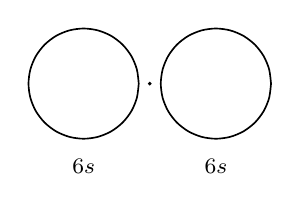
\begin{tikzpicture}[scale=0.7]
                            \footnotesize
                            \filldraw [semithick,fill=white] plot[domain=0:2*pi,smooth,variable=\thta] ({\thta r}:1);
                            \filldraw [semithick,fill=white,xshift=2.4cm] plot[domain=0:2*pi,smooth,variable=\thta] ({\thta r}:1);
                            \fill (1.2,0) circle (1pt);

                            \node at (0,-1.5) {$6s$};
                            \node at (2.4,-1.5) {$6s$};
                        \end{tikzpicture}\\[1.5em]
                        \begin{tikzpicture}[scale=0.7]
                            \footnotesize
                            \filldraw [semithick,fill=grt] ({-6^0.5/4},0,0) circle (6^0.5/4);
                            \filldraw [semithick,fill=white] ({6^0.5/4},0,0) circle (6^0.5/4);
                            \filldraw [semithick,fill=grt,xshift=2.8cm] ({6^0.5/4},0,0) circle (6^0.5/4);
                            \filldraw [semithick,fill=white,xshift=2.8cm] ({-6^0.5/4},0,0) circle (6^0.5/4);
                            \fill (1.4,0) circle (1pt);

                            \node at (0,-1) {$5p$};
                            \node at (2.8,-1) {$5p$};
                        \end{tikzpicture}\\[1.5em]
                        \begin{tikzpicture}[scale=0.7]
                            \footnotesize
                            \begin{scope}[rotate=-90]
                                \filldraw [semithick,fill=white] plot [domain=0.63:2.51,smooth,variable=\thta] ({\thta r}:{0.5*2.5^0.5*(3*sin(\thta r)^2-1)});
                                \filldraw [semithick,fill=white] plot [domain=3.75:5.67,smooth,variable=\thta] ({\thta r}:{0.5*2.5^0.5*(3*sin(\thta r)^2-1)});
                                \filldraw [semithick,fill=grt] (-0.4,0,0) arc[start angle=120,end angle=60,x radius=0.8cm,y radius=0.9cm] arc[start angle=-60,end angle=-120,x radius=0.8cm,y radius=0.9cm];
                            \end{scope}
                            \begin{scope}[rotate=-90,yshift=3.5cm]
                                \filldraw [semithick,fill=white] plot [domain=0.63:2.51,smooth,variable=\thta] ({\thta r}:{0.5*2.5^0.5*(3*sin(\thta r)^2-1)});
                                \filldraw [semithick,fill=white] plot [domain=3.75:5.67,smooth,variable=\thta] ({\thta r}:{0.5*2.5^0.5*(3*sin(\thta r)^2-1)});
                                \filldraw [semithick,fill=grt] (-0.4,0,0) arc[start angle=120,end angle=60,x radius=0.8cm,y radius=0.9cm] arc[start angle=-60,end angle=-120,x radius=0.8cm,y radius=0.9cm];
                            \end{scope}
                            \fill (1.75,0) circle (1pt);

                            \node at (0,-1) {$5d$};
                            \node at (3.5,-1) {$5d$};
                        \end{tikzpicture}
                    \end{center}
                \end{proof}
                \item Show how the group orbitals and the central atom would interact.
                \begin{proof}[Answer]
                    ${\color{white}hi}$
                    \begin{center}
                        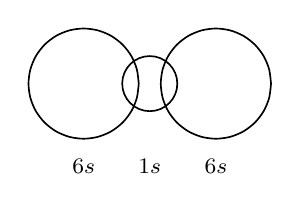
\begin{tikzpicture}[scale=0.7]
                            \footnotesize
                            \filldraw [semithick,fill=white] plot[domain=0:2*pi,smooth,variable=\thta] ({\thta r}:1);
                            \filldraw [semithick,fill=white,xshift=2.4cm] plot[domain=0:2*pi,smooth,variable=\thta] ({\thta r}:1);
                            \draw [semithick] (1.2,0) circle (5mm);

                            \node at (0,-1.5) {$6s$};
                            \node at (1.2,-1.5) {$1s$};
                            \node at (2.4,-1.5) {$6s$};
                        \end{tikzpicture}\\[1.5em]
                        \begin{tikzpicture}[scale=0.7]
                            \footnotesize
                            \filldraw [semithick,fill=grt] ({-6^0.5/4},0,0) circle (6^0.5/4);
                            \filldraw [semithick,fill=white] ({6^0.5/4},0,0) circle (6^0.5/4);
                            \filldraw [semithick,fill=grt,xshift=2.8cm] ({6^0.5/4},0,0) circle (6^0.5/4);
                            \filldraw [semithick,fill=white,xshift=2.8cm] ({-6^0.5/4},0,0) circle (6^0.5/4);
                            \draw [semithick] (1.4,0) circle (5mm);

                            \node at (0,-1) {$5p$};
                            \node at (1.4,-1) {$1s$};
                            \node at (2.8,-1) {$5p$};
                        \end{tikzpicture}\\[1.5em]
                        \begin{tikzpicture}[scale=0.7]
                            \footnotesize
                            \begin{scope}[rotate=-90]
                                \filldraw [semithick,fill=white] plot [domain=0.63:2.51,smooth,variable=\thta] ({\thta r}:{0.5*2.5^0.5*(3*sin(\thta r)^2-1)});
                                \filldraw [semithick,fill=white] plot [domain=3.75:5.67,smooth,variable=\thta] ({\thta r}:{0.5*2.5^0.5*(3*sin(\thta r)^2-1)});
                                \filldraw [semithick,fill=grt] (-0.4,0,0) arc[start angle=120,end angle=60,x radius=0.8cm,y radius=0.9cm] arc[start angle=-60,end angle=-120,x radius=0.8cm,y radius=0.9cm];
                            \end{scope}
                            \begin{scope}[rotate=-90,yshift=3.5cm]
                                \filldraw [semithick,fill=white] plot [domain=0.63:2.51,smooth,variable=\thta] ({\thta r}:{0.5*2.5^0.5*(3*sin(\thta r)^2-1)});
                                \filldraw [semithick,fill=white] plot [domain=3.75:5.67,smooth,variable=\thta] ({\thta r}:{0.5*2.5^0.5*(3*sin(\thta r)^2-1)});
                                \filldraw [semithick,fill=grt] (-0.4,0,0) arc[start angle=120,end angle=60,x radius=0.8cm,y radius=0.9cm] arc[start angle=-60,end angle=-120,x radius=0.8cm,y radius=0.9cm];
                            \end{scope}
                            \draw [semithick] (1.75,0) circle (5mm);

                            \node at (0,-1) {$5d$};
                            \node at (1.75,-1) {$1s$};
                            \node at (3.5,-1) {$5d$};
                        \end{tikzpicture}
                    \end{center}
                \end{proof}
                \item Which interaction would you expect to be the strongest, and why?
                \begin{proof}[Answer]
                    The $d_{z^2}$ interaction should be the strongest. In the MO energy diagram for \ce{MH6} bonding, the hydrogen orbitals are closest in energy to the metal $d$ orbitals. It stands to reason that it would be similar for square pyramidal bonding and deuterium.
                \end{proof}
            \end{enumerate}
        \end{enumerate}
    \end{enumerate}
    \newpage
    \item We derived in class the MO diagram for \ce{Re2Cl8^2-}, a complex with a \ce{Re-Re} quadruple bond. Two chloride ligands on each \ce{Re} can be replaced with two (neutral) \ce{PMe2Ph} ligands to give the cationic complex \ce{Re2(PMe2Ph)4Cl4^2+}, which has a similar $\sigma^2\pi^4\delta^2$ electronic configuration and a \ce{Re-Re} quadruple bond of $\SI{2.215}{\angstrom}$ in length. The 1-electron and 2-electron reduced species \ce{Re2(PMe2Ph)4Cl4^+} and \ce{Re2(PMe2Ph)4Cl4} can be prepared, and their structures show \ce{Re-Re} bond lengths of $\SI{2.218}{\angstrom}$ and $\SI{2.241}{\angstrom}$, respectively. Give the electronic configurations for the 1- and 2-electron reduced species (as given above for the unreduced species), and suggest how this could account for the different \ce{Re-Re} bond lengths in the three compounds.
    \begin{proof}[Answer]
        From the MO diagram discussed in lecture, we know that adding more electrons to a complex isoelectronic to \ce{Re2Cl8^2-} will begin to occupy the $\delta^*$ molecular orbitals. Thus, the electronic configuration of \ce{Re2(PMe2Ph)4Cl4^+} is $\sigma^2\pi^4\delta^2{\delta^*}^1$, and the electronic configuration of \ce{Re2(PMe2Ph)4Cl4} is $\sigma^2\pi^4\delta^2{\delta^*}^2$.\par
        Because the increasingly reduced species have increasing antibonding character, it stands to reason that the bond will weaken and lengthen.
    \end{proof}
\end{enumerate}




\end{document}